\documentclass[%
class = book,%
crop = false,%
float = true,%
multi = true,%
preview = false,%
]{standalone}
\usepackage[%
    backend    = biber,%
    style      = chem-acs,%
    autocite   = superscript,%
    backref    = true,%
    biblabel   = brackets,%
    doi        = true,%
    minnames   = 1,%
    maxnames   = 999,%
]{biblatex}
\let\cite\autocite
\DefineBibliographyStrings{english}{%
  backrefpage = {page},% originally "cit. on p."
  backrefpages = {pages},
}
\addbibresource{./paper_04/paper.bib}
\addbibresource{./paper_05/tutorial.bib}
\addbibresource{./library2.bib}
\onlyifstandalone{\usepackage{amsmath}}
\onlyifstandalone{\usepackage[usenames,dvipsnames,svgnames,hyperref,table]{xcolor}}
\onlyifstandalone{\definecolor{carmine}{HTML}{960018}}
\usepackage{booktabs}
\usepackage{braket}
\usepackage{cancel}
% https://tex.stackexchange.com/q/105902/94717
% \newcommand\Ccancel[2][black]{\renewcommand\CancelColor{\color{#1}}\cancel{#2}}
\newcommand\Ccancelto[3][black]{\renewcommand\CancelColor{\color{#1}}\cancelto{#2}{#3}}
\onlyifstandalone{\usepackage[margin=1in]{geometry}}
\onlyifstandalone{\raggedbottom}
\usepackage{graphicx}
\onlyifstandalone{\usepackage{hyperref}}
\onlyifstandalone{\usepackage{setspace}}
\usepackage[%
    separate-uncertainty = true,%
    multi-part-units = single,%
    range-units = single,%
    retain-explicit-plus = true,%
]{siunitx}
\DeclareSIUnit\au{a.u.}
\usepackage{tabulary}
\usepackage{xspace}
\newcommand\hf{Hartree\textendash{}Fock\xspace}%
\newcommand{\caps}[1]{\uppercase{#1}}
\begin{document}
\chapter{Introduction}
\label{ch:introduction}

\section{\texorpdfstring{\caps{Introduction to the thesis}}{Introduction to the thesis}}

The unifying theme of this thesis is that it is possible to identify the contribution of specific intermolecular interactions to spectroscopic response. The contributions of specific intermolecular interactions are in the language of energy decomposition analysis using absolutely localized molecular orbitals, abbreviated as ALMO-EDA. The necessary background for ALMO-EDA is given in sections~\ref{sec:introduction}.

The majority of this thesis presents applications of response theory to calculating spectroscopic properties, specifically vibrational frequencies in chapters~\ref{ch:anions}, \ref{ch:paper_02}, \ref{ch:paper_03} and dipole polarizabilities in chapter~\ref{ch:paper_04}, where each property is decomposed in terms of contributions to the final response from distorting the molecular geometry, allowing the non-interacting molecular densities to interact and then relax, and finally allowing charge to flow unrestricted between molecules. Chapter~\ref{ch:paper_05} presents a new model for implementing quantum chemical methods, with the first dipole hyperpolarizability as an example (sections~\ref{paper_05:ssec:hyperpolarizability_reference_implementation}~and~\ref{paper_05:ssec:hyperpolarizability_tutorial}), and how decomposition of molecular properties may be implemented and disseminated in the future.

The remainder of this introduction will cover the basic language of molecular response theory and its connection to macroscopic spectroscopic observables, covering examples of which observables are related to which microscopic terms (section~\ref{sec:connection-between-macroscopic-and-microscopic}). It will also cover more general cases of how those microscopic terms appear in different forms of derivation, all of which are related and give identical final answers. Specifically, a connection will be made between phenomenological Hamiltonians (section~\ref{ssec:phenomenological-approach}), series expansions (section~\ref{ssec:series-expansion}), energy derivatives (sections~\ref{ssec:derivative-evaluation},~\ref{ssec:finite-difference-for-numerical-derivatives},~and~\ref{ssec:analytic-derivative-theory}), perturbation theory (section~\ref{ssec:perturbation-theory}), and the polarization propagator (section~\ref{sec:dynamic-properties}), of which the latter two are appropriate for incorporation of time dependence, leading to dynamic properties.

\section{\texorpdfstring{\caps{Connection between macroscopic and microscopic properties}}{Connection between macroscopic and microscopic properties}}
\label{sec:connection-between-macroscopic-and-microscopic}

\begin{table}
  \centering
  \caption[Connection between specific energy derivatives and their respective molecular properties]{Connection between specific energy derivatives and their respective molecular properties. \(F\) is an applied electric field, \(B\) is an applied magnetic field, \(X\) is a nuclear coordinate, \(m\) is a nuclear magnetic moment, \(J\) is a total rotational moment, \(I\) is a nuclear spin, and \(S\) is the intrinsic electronic spin. Adapted from Ref.~\parencite{gauss2000}.\label{tab:gauss}}
  \begin{tabulary}{0.85\textwidth}{rL}
    \toprule
    \textbf{Energy derivative} & \textbf{Molecular property} \\
    \midrule
    \(\frac{dE}{dF_{i}}\)                          & dipole moment; in a similar manner also multipole moments, electric field gradients, etc. \\
    \(\frac{d^{2}E}{dF_{\alpha}dF_{\beta}}\)       & polarizability \\
    \(\frac{d^{3}E}{dF_{\alpha}d^{2}F_{\beta}}\)   & (first) hyperpolarizability \\
    \(\frac{dE}{dX_{i}}\)                          & forces on nuclei; stationary points on potential energy surfaces, equilibrium and transition state structures \\
    \(\frac{d^{2}E}{dX_{i}dX_{j}}\)                & harmonic force constants; harmonic vibrational frequencies \\
    \(\frac{d^{3}E}{dX_{i}dX_{j}dX_{k}}\)          & cubic force constants; vibrational corrections to distances and rotational constants \\
    \(\frac{d^{4}E}{dX_{i}dX_{j}dX_{k}dX_{l}}\)    & quartic force constants; anharmonic corrections to vibrational frequencies \\
    \(\frac{d^{2}E}{dX_{i}dF_{\alpha}}\)           & dipole derivatives; infrared intensities within the harmonic approximation \\
    \(\frac{d^{3}E}{dX_{i}dF_{\alpha}dF_{\beta}}\) & polarizability derivative; Raman intensities \\
    \(\frac{d^{2}E}{dB_{\alpha}dB_{\beta}}\)       & magnetizability \\
    \(\frac{d^{2}E}{dm_{K_{j}}dB_{\alpha}}\)       & nuclear magnetic shielding tensor; relative NMR shifts \\
    \(\frac{d^{2}E}{dI_{K_{i}}dI_{L_{j}}}\)        & indirect spin-spin coupling constant \\
    \(\frac{d^{2}E}{dB_{\alpha}dJ_{\beta}}\)       & rotational \textit{g}-tensor; rotational spectra in magnetic field \\
    \(\frac{d^{2}E}{dI_{K_{i}}dB_{\alpha}}\)       & nuclear spin-rotation tensor; fine structure in rotational spectra \\
    \(\frac{dE}{dm_{K_{j}}}\)                      & spin density; hyperfine interaction constants \\
    \(\frac{d^{2}E}{dS_{i}dB_{\alpha}}\)           & electronic \textit{g}-tensor \\
    \bottomrule
  \end{tabulary}
\end{table}

% The experimentalist works at the macroscopic level and typically records the reponse of the electromagnetic field.
% The theoretician works at the microscopic level and typically calculates the molecular response.

There is often a direct connection between the macroscopic observables measurable by spectroscopic techniques and the molecular response calculated at the microscopic scale. Tables~\ref{tab:gauss}~and~\ref{tab:norman} give examples of the most common molecular properties of interest and their relationships to energy derivatives and response functions, respectively. Although there is often quite some distance in terms of mathematical derivation and code development effort between

Poles and residues

residues lead to transition moments

A residue analysis provides a mean to obtain \textit{excited state properties} from the ground state response function. The poles equal excitation energies and the residues are given by
\begin{equation*}
  \lim_{\omega_{1} \to \omega_{n0}} (\omega_{n0} - \omega_{1}) \braket{\braket{\hat{P};\hat{Q}^{\omega_{1}}}} = \braket{0|\hat{P}|n} \braket{n|\hat{Q}^{\omega_{1}}|0}
\end{equation*}
Spin-orbit coupling constants between singlet/triplet states correspond to the residue of the triplet linear response function:
\begin{equation*}
  \lim_{\omega \to \omega_{f}} (\omega - \omega_{f}) \braket{\braket{\hat{H}_{\text{so}};\hat{V}^{\omega_{f}}}}
\end{equation*}

More appropriate for time- or frequency-dependent response properties

\begin{table}
  \centering
  \caption[Connection between specific response functions and their respective molecular properties]{Connection between specific (non)linear response functions and their respective molecular properties. Adapted from Ref.~\parencite{C1CP21951K}.\label{tab:norman}}
  \begin{tabular}{lll}
    \toprule
    \textbf{Molecular Property}       & \textbf{Definition}                                                                    & \textbf{Type of response function} \\
    \midrule
    polarizability                    & \( \braket{\braket{\hat{\mu};\hat{\mu}}}_{\omega} \)                                   & linear \\
    magnetizability                   & \( \braket{\braket{\hat{m};\hat{m}}}_{0} \)                                            & linear \\
    optical rotation                  & \( \braket{\braket{\hat{\mu};\hat{m}}}_{\omega} \)                                     & linear \\
    electronic circular dichroism     & \( \braket{\braket{\hat{\mu};\hat{m}}}_{\omega_{f}} \)                                 & single residue of linear \\
    IR intensities                    & \( \braket{\braket{\hat{\mu};\partial\hat{H}_{0}/\partial R}}_{\omega} \)              & linear \\
    NMR spin-spin coupling constants  & \( \braket{\braket{\hat{h}_{\text{SD}};\hat{h}_{\text{SD}}}}_{0} \),                   & linear \\
                                      & \( \braket{\braket{\hat{h}_{\text{FC}};\hat{h}_{\text{FC}}}}_{0} \),                   & linear \\
                                      & \( \braket{\braket{\hat{h}_{\text{PSO}};\hat{h}_{\text{PSO}}}}_{0} \)                  & linear \\
    NMR chemical shifts               & \( \braket{\braket{\hat{l}_{O};\hat{h}_{\text{PSO}}}}_{0} \)                           & linear \\
    EPR \textit{g}-tensor             & \( \braket{\braket{\hat{l}_{O};\hat{h}_{\text{SOC}}}}_{0} \)                           & linear \\
    \midrule
    static first hyperpolarizability  & \( \braket{\braket{\hat{\mu};\hat{\mu},\hat{\mu}}}_{0,0} \)                            & quadratic \\
    second-harmonic generation        & \( \braket{\braket{\hat{\mu};\hat{\mu},\hat{\mu}}}_{\omega,\omega} \)                  & quadratic \\
    electro-optical Pockels effect    & \( \braket{\braket{\hat{\mu};\hat{\mu},\hat{\mu}}}_{\omega,0} \)                       & quadratic \\
    optical rectification             & \( \braket{\braket{\hat{\mu};\hat{\mu},\hat{\mu}}}_{\omega,-\omega} \)                 & quadratic \\
    Faraday rotation                  & \( \braket{\braket{\hat{\mu};\hat{\mu},\hat{m}}}_{\omega,0} \)                         & quadratic ? \\
    magnetic circular dichroism       & \( \braket{\braket{\hat{\mu};\hat{\mu},\hat{m}}}_{\omega_{f},0} \)                     & () residue of quadratic \\
    Raman intensities                 & \( \braket{\braket{\hat{\mu};\hat{\mu},\partial\hat{H}_{0}/\partial R}}_{\omega,0} \)  & quadratic \\
    \midrule
    static second hyperpolarizability & \( \braket{\braket{\hat{\mu};\hat{\mu},\hat{\mu},\hat{\mu}}}_{0,0,0} \)                & cubic \\
    third-harmonic generation         & \( \braket{\braket{\hat{\mu};\hat{\mu},\hat{\mu},\hat{\mu}}}_{\omega,\omega,\omega} \) & cubic \\
    \bottomrule
  \end{tabular}
\end{table}

\section{\texorpdfstring{\caps{Static (time-independent) response properties}}{Static (time-independent) response properties}}
\label{sec:static-properties}

TODO

Sources: Toulouse; Handy has expressions for derivatives leading to integrals

Two possible ways to perform the derivation:

\begin{enumerate}
\item from series expansion of the energy with respect to one or more perturbations (section~\ref{ssec:series-expansion})
\item from a phenomenological Hamiltonian (sort of like the correspondence principle, quantizing a classical expression) (section~\ref{ssec:phenomenological-approach})
\end{enumerate}

\subsection{Phenomenological approach}
\label{ssec:phenomenological-approach}

For a one-dimensional spring connecting a ball to a fixed object, Hooke's law is
\begin{equation}
  \label{eq:hooke_1d}
  F = -k x,
\end{equation}
where \(x\) is the displacement of the spring from equilibrium in meters, \(k\) is the spring constant in units of \si{\newton\per\meter}, and \(F\) is the restoring force in units of newtons acting on the displaced spring by the object it is attached to. If the sign is reversed, then the equation can be viewed as describing the force of spring acting on the attached object; it is a direction change and a matter of convention.

Hooke's law can be generalized to multiple dimensions. For example, in three-dimensional space it can be written as
\begin{equation}
  \label{eq:force_hooke_matrix}
  \begin{bmatrix}
    F_{1} \\ F_{2} \\ F_{3}
  \end{bmatrix}
  = -
  \begin{bmatrix}
    k_{11} & k_{12} & k_{13} \\
    k_{21} & k_{22} & k_{23} \\
    k_{31} & k_{32} & k_{33}
  \end{bmatrix}
  \begin{bmatrix}
    x_{1} \\ x_{2} \\ x_{3}
  \end{bmatrix},
\end{equation}
which can represent either a single object or three one-dimensional springs. It can also be made \(3N\)-dimensional when describing the forces on \(N\) atoms (each with 3 Cartesian components) given their relative positions \(\mathbf{x}\) and the ``stiffness'' of their connectivity \(\mathbf{k}\). In the most general \(N\)-dimensional form, it can be written as
\begin{equation}
  \label{eq:force_hooke_sum}
  F_{i} = - \sum_{j}^{N} k_{ij} x_{j},
\end{equation}
or in Einstein summation notation where repeated indices are implicitly summed (contracted) over as
\begin{equation}
  \label{eq:force_hooke_einstein}
  F_{i} = -k_{ij} x_{j},
\end{equation}
where both \(i,j\) range from 1 to \(N\), leading to vectors \(\mathbf{F}\) and \(\mathbf{x}\) of shape \([N]\) and a matrix \(\mathbf{k}\) of shape \([N,N]\). From \eqref{eq:force_hooke_matrix}, \eqref{eq:force_hooke_sum}, and \eqref{eq:force_hooke_einstein}, if off-diagonal elements of \(k\) are allowed to be nonzero, there can be coupling between springs. For example, if \(i \leftarrow 1\), in the case of coupling,
\begin{equation}
  \label{eq:force_hooke_example}
  F_{1} = -(k_{11}x_{1} + k_{12}x_{2} + k_{13}x_{3}),
\end{equation}
which reduces to
\begin{equation}
  \label{eq:force_hooke_example_nocoupling}
  F_{1} = -k_{11}x_{1}
\end{equation}
in the absence of coupling, or the same result obtained in \eqref{eq:hooke_1d}.

The force is also related to the energy. In one dimension,
\begin{align}
  \label{eq:energy_derivative_1d}
  F &= \nabla E \\
  &= \frac{\partial E}{\partial x},
\end{align}
where \(\nabla \equiv \partial/\partial x\). For convenience, the negative sign will be dropped from the remainder of the derivation. In \(N\) dimensions, like \eqref{eq:force_hooke_einstein}, \eqref{eq:energy_derivative_1d} is (using vector calculus)
\begin{equation}
  \label{eq:force_partial_derivative}
  F_{i} = \frac{\partial E}{\partial x_{i}}.
\end{equation}

Equating the \(F_{i}\) in \eqref{eq:force_hooke_einstein} and \eqref{eq:force_partial_derivative} gives
\begin{equation}
  \label{eq:equated_force}
  k_{ij} x_{j} = \frac{\partial E}{\partial x_{i}}.
\end{equation}

To solve for the stiffness coefficients, take the partial derivative of both sides with respect to \(x_{j}\), using the product rule on the left hand side:
\begin{align}
  \label{eq:hooke_derivation_1}
  \left( \frac{\partial}{\partial x_{j}} \right) \left( k_{ij} x_{j} \right) &= \left( \frac{\partial}{\partial x_{j}} \right) \left( \frac{\partial E}{\partial x_{i}} \right) \\
  \label{eq:hooke_derivation_2}
  \Ccancelto[carmine]{0}{\left[ \left( \frac{\partial}{\partial x_{j}} \right) \left( k_{ij} \right) \right]} x_{j} + k_{ij} \Ccancelto[Green]{1}{\left[ \left( \frac{\partial}{\partial x_{j}} \right) x_{j} \right]} &= \frac{\partial^{2} E}{\partial x_{j} \partial x_{i}} \\
  \label{eq:hooke_derivation_3}
  k_{ij} &= \frac{\partial^{2} E}{\partial x_{j} \partial x_{i}}.
\end{align}

This tells that the internal stiffness is related to the second derivative of the energy with respect to nuclear coordinate displacements. The internal stiffness matrix is the molecular Hessian, where each ``spring constant'' is called a force constant, which describes how a change or perturbation to one atomic coordinate affects a change in another atomic coordinate.

Wikipedia: symmetry of second derivatives, Euler's (interchange) theorem, TODO this may only be for real perturbations.
\begin{equation}
  \frac{\partial^{2} E}{\partial x_{j} \partial x_{i}} = \frac{\partial^{2} E}{\partial x_{i} \partial x_{j}}
\end{equation}

A similar derivation holds for the dipole polarizability, \(\alpha\), which is the ratio of the induced dipole moment \(\mu\) of a system to the electric field \(F\) that produces this dipole moment. Both \(\mu\) and \(F\) are 3-dimensional vector quantities,
\begin{equation}
  \label{eq:phenomenological-polarizability}
  \vec{\mu} = \vec{\vec{\alpha}} \cdot \vec{F},
\end{equation}
which can be expanded identically to \eqref{eq:force_hooke_matrix} as
\begin{equation}
  \begin{bmatrix}
    \mu_{1} \\ \mu_{2} \\ \mu_{3}
  \end{bmatrix}
  =
  \begin{bmatrix}
    \alpha_{11} & \alpha_{12} & \alpha_{13} \\
    \alpha_{21} & \alpha_{22} & \alpha_{23} \\
    \alpha_{31} & \alpha_{32} & \alpha_{33}
  \end{bmatrix}
  \begin{bmatrix}
    F_{1} \\ F_{2} \\ F_{3},
  \end{bmatrix}
\end{equation}
or in Einstein summation notation as
\begin{equation}
  \label{eq:polarizability_einstein}
  \mu_{i} = \alpha_{ij} F_{j}.
\end{equation}
This is the most general case, where anisotropy may be present in the polarizability tensor, leading to nonzero off-diagonal elements.

Another definition of the molecular dipole moment induced by an external (applied) electric field is
\begin{equation}
  \label{eq:dipole_from_derivative}
  \mu_{i} = \frac{\partial E}{\partial F_{i}}.
\end{equation}
Following \eqref{eq:equated_force}, equating \eqref{eq:polarizability_einstein} and \eqref{eq:dipole_from_derivative} gives
\begin{equation}
  \label{eq:equated_polarizability}
  \alpha_{ij} F_{j} = \frac{\partial E}{\partial F_{i}}
\end{equation}
The remaining steps follow identically to \eqref{eq:hooke_derivation_1}, \eqref{eq:hooke_derivation_2}, and \eqref{eq:hooke_derivation_3}:
\begin{align}
  \left( \frac{\partial}{\partial F_{j}} \right) \left( \alpha_{ij} F_{j} \right) &= \left( \frac{\partial}{\partial F_{j}} \right) \left( \frac{\partial E}{\partial F_{i}} \right) \\
  \Ccancelto[carmine]{0}{\left( \frac{\partial \alpha_{ij}}{\partial F_{j}} \right)} F_{j} + \alpha_{ij} \Ccancelto[Green]{1}{\left( \frac{\partial F_{j}}{\partial F_{j}} \right)} &= \frac{\partial^{2} E}{\partial F_{j} \partial F_{i}} \\
  \alpha_{ij} &= \frac{\partial^{2} E}{\partial F_{j} \partial F_{i}}
\end{align}

\subsection{Series expansion}
\label{ssec:series-expansion}
TODO this is not quite right because it doesn't handle higher-order cross-terms properly!

More correctly, the derivative terms in section~\ref{ssec:phenomenological-approach} originate from series expansions of the energy in the presence of a perturbation; for \eqref{eq:hooke_1d}, it is internal geometric displacements, and in \eqref{eq:phenomenological-polarizability} it is an external electric field. The energy in the presence of an arbitrary perturbation \(P\) is written as
\begin{equation}
  \label{eq:taylor-expansion}
  \begin{aligned}
    E(P) &= \sum_{n = 0}^{\infty} \frac{1}{n!} \left. \frac{\partial^{n} E}{\partial P^{n}} \right|_{P = a} \cdot (P - a)^{n} \\
    &= \sum_{n = 0}^{\infty} \frac{1}{n!} E^{(n)}(a) \cdot (P - a)^{n} \\
    &= E^{(0)}(a) + E^{(1)}(a) \cdot (P - a) + \frac{1}{2} E^{(2)}(a) \cdot (P - a)^{2} + \frac{1}{6} E^{(3)}(a) \cdot (P - a)^{3} + \cdots ,
  \end{aligned}
\end{equation}
where \(a\) is the point at which the derivative is taken. Choosing \(a \overset{!}{=} 0\) turns the Taylor series into a Maclaurin series:
\begin{equation}
  \label{eq:maclaurin-expansion}
  \begin{aligned}
    E(P) &= \sum_{n = 0}^{\infty} \frac{1}{n!} \left. \frac{\partial^{n} E}{\partial P^{n}} \right|_{P = 0} \cdot P^{n} \\
    &= \sum_{n = 0}^{\infty} \frac{1}{n!} E^{(n)} \cdot P^{n} \\
    &= E^{(0)} + E^{(1)} \cdot P + \frac{1}{2} E^{(2)} \cdot P^{2} + \frac{1}{6} E^{(3)} \cdot P^{3} + \cdots
  \end{aligned}
\end{equation}
The perturbation \(P\) may have multiple components. For example, there are 3 possible Cartesian components to an external electric field \(\mathbf{F} = (F_{x}, F_{y}, F_{z})\) and \(3N\) atomic coordinates. Generalizing the dimensionality of \(P\) to \(k\) and inserting into \eqref{eq:maclaurin-expansion} gives
\begin{equation}
  \label{eq:maclaurin-expansion-vector}
  \begin{aligned}
    E(\mathbf{P}) &= \sum_{n = 0}^{\infty} \sum_{i = 1}^{k} \frac{1}{n!} \left. \frac{\partial^{n} E}{\partial P_{i}^{n}} \right|_{P_{i} = 0} \cdot P_{i}^{n} \\
    &= \sum_{n = 0}^{\infty} \sum_{i = 1}^{k} \frac{1}{n!} E_{i}^{(n)} \cdot P_{i}^{n} \\
    &= E^{(0)} + \left[ (E_{1}^{(1)} \cdot P_{1}) + (E_{2}^{(1)} \cdot P_{2}) + \cdots + (E_{k}^{(1)} \cdot P_{k}) \right] \\
    &\quad + \frac{1}{2} \left[ (E_{1}^{(2)} \cdot P_{1}^{2}) + (E_{2}^{(2)} \cdot P_{2}^{2}) + \cdots + (E_{k}^{(2)} \cdot P_{k}^{2}) \right] + \cdots
  \end{aligned}
\end{equation}

Considering specific examples, using \eqref{eq:maclaurin-expansion-vector}, replacing \(\mathbf{P}\) with an external electric field \(\mathbf{F}\), and switching to Einstein notation gives
\begin{equation}
  \label{eq:electric-field-expansion}
  E(\mathbf{F}) = E_{0} + \mu_{i} \cdot F_{i} + \frac{1}{2} \alpha_{ij} \cdot F_{i}F_{j} + \frac{1}{6} \beta_{ijk} \cdot F_{i}F_{j}F_{k} + \frac{1}{24} \gamma_{ijkl} \cdot F_{i}F_{j}F_{k}F_{l} + \cdots
\end{equation}

\subsection{Derivative evaluation}
\label{ssec:derivative-evaluation}

Up to this point, it has not been necessary to specify which energy expression is being differentiated: it is the energy expression for the chosen method (HF, \(\omega\)B97M-V, MP2, CCSD(T), \dots). These derivatives may be evaluated in one of two ways:
\begin{enumerate}
\item numerically, by using a finite difference expression (usually based on central differences) for the desired derivative order, evaluating the energy at multiple perturbation strengths (step sizes) and directions, or
\item analytically, by differentiating the energy expression ``on paper'' and evaluating it directly.
\end{enumerate} %TODO identify terms in the Raman perturbation or alter the Gauss table
It is also possible to combine numerical and analytic approaches to obtain higher-order derivatives. For example, in the calculation of Raman intensities, defined as \(\frac{\partial^{3} E}{\partial X_{A} \partial F_{i} \partial F_{j}}\), there are six unique ways to perform the derivative, shown in Table~\ref{tab:raman-unique-derivatives}.
\begin{table}
  \centering
  \begin{singlespace}
    \begin{tabular}{ccc}
      \toprule
      \(X_{A}\) & \(F_{i}\) & \(F_{j}\) \\
      \midrule
      a & a & a \\
      a & a & n \\
      \cancel{a} & \cancel{n} & \cancel{a} \\
      n & a & a \\
      a & n & n \\
      n & a & n \\
      \cancel{n} & \cancel{n} & \cancel{a} \\
      n & n & n \\
      \bottomrule
    \end{tabular}
  \end{singlespace}
  \caption[Possible analytic and numerical permutations for Raman intensities]{Possible permutations of analytic (a) and numerical (n) differentiation for each perturbation term in calculating Raman intensities. The two cancelled entries are not unique due to permutational symmetry.}
  \label{tab:raman-unique-derivatives}
\end{table}
More explicitly, the first row corresponds to a fully analytic third derivative, the next three rows correspond to first-order finite difference of analytic second derivatives, the next three rows correspond to second-order finite difference of analytic first derivatives, and the last row corresponds to the third-order finite difference of energies. Due to symmetry in the electric field perturbation indices, two of the eight permutations are identical to others already present; for example, a/a/n and a/n/a are functionally identical.

In practice, the fully analytic third derivative is not usually implemented, but second derivatives are, leading to two unique possibilities:
\begin{align}
  \label{eq:raman-intensity-from-polarizability}
  \frac{\partial^{3} E}{\partial X_{A} \partial F_{i} \partial F_{j}} &= \underbrace{\frac{\partial}{\partial X_{A}}}_{\text{numeric}} \underbrace{\left(\frac{\partial^{2} E}{\partial F_{i} \partial F_{j}}\right)}_{\text{analytic}} = \frac{\partial \alpha_{ij}}{\partial X_{A}}, \\
  \label{eq:raman-intensity-from-dipgrad}
  &= \underbrace{\frac{\partial}{\partial F_{i}}}_{\text{numeric}} \underbrace{\left(\frac{\partial^{2} E}{\partial X_{A} \partial F_{j}}\right)}_{\text{analytic}} = \frac{\partial}{\partial F_{i}} \left( \frac{\partial \mu_{j}}{\partial X_{A}} \right).
\end{align}
In \eqref{eq:raman-intensity-from-polarizability} there are \(2 \times (3N \,\,\text{atomic coordinates}) = 6N\) atom-displaced polarizability calculations. This is closer to the textbook definition of Raman intensities, which are the change in molecular polarizability along each normal mode coordinate\cite{TODO}. In \eqref{eq:raman-intensity-from-dipgrad}, the dipole gradient (needed for IR intensities) is calculated analytically for \(2 \times (3 \,\,\text{field directions}) = 6\) finite electric field calculations.
% In \eqref{eq:raman-intensity-from-polarizability}, the polarizability is calculated analytically for each nuclear displacement, leading to \(2 \times (3N \,\,\text{atomic coordinates}) = 6N\) atom-displaced polarizability calculations. This is closer to the textbook definition of Raman intensities, which are the change in molecular polarizability along each normal mode coordinate\cite{TODO}. In \eqref{eq:raman-intensity-from-dipgrad}, the dipole gradient (needed for IR intensities) is calculated analytically for \(2 \times (3 \,\,\text{field directions}) = 6\) finite electric field calculations.

\subsection{Finite difference for numerical derivatives}
\label{ssec:finite-difference-for-numerical-derivatives}

% \begin{itemize}
% \item calculation time
% \item uncoupled and perturbative approximations to fully iterative results
% \item lack of finite-difference error
% \item frequency-dependent perturbations
% \item response to applied magnetic fields without complex energies
% \end{itemize}
% As discussed in section~\ref{ssec:decomp-line-resp} and ref.~\parencite{gauss2000}, there are considerable disadvantages to performing numerical differentiation of the wavefunction. The most commonly encountered disadvantage is calculation time: compared to a single closed-form calculation, external (electric and magnetic) field perturbations require 6 additional calculations for each derivative order, and those depending on nuclear displacements require \(6N\) additional calculations. Admittedly, it is difficult to compare calculation time further since the cost of analytic methods is not independent of system size, but the

As discussed in section~\ref{ssec:decomp-line-resp} and ref.~\parencite{gauss2000}, there are considerable disadvantages to performing numerical differentiation of the wavefunction.

TODO numerical noise in figure~\ref{fig:finite-difference-numerical-noise}

\begin{figure}
  \centering
  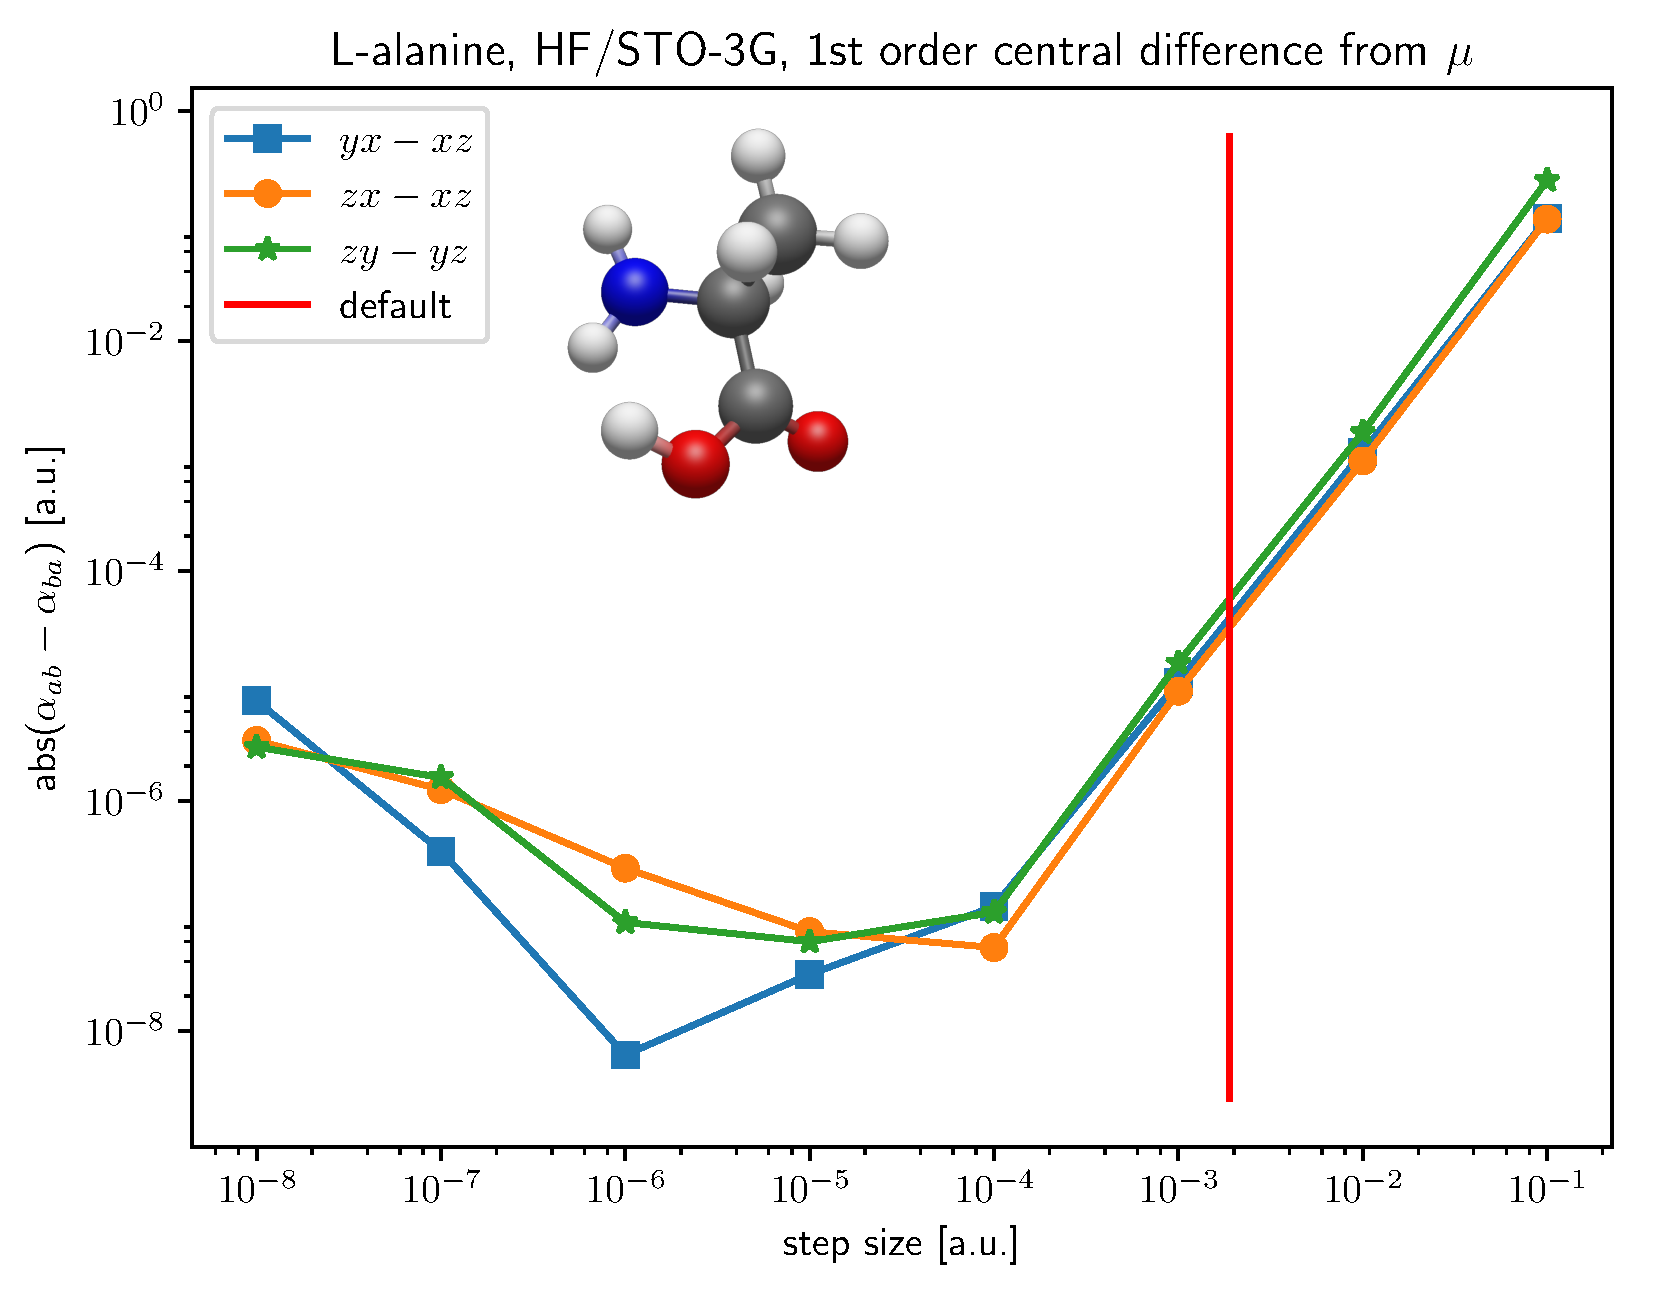
\includegraphics[width=\textwidth]{./diff_overlay.pdf}
  \caption[Asymmetry in the 1st-order finite-difference polarizability]{Effect of numerical noise on the off-diagonal matrix elements of the polarizability tensor. Nonzero differences indicate asymmetry, and the polarizability tensor is supposed to be symmetric. The red bar indicates the default step size for the applied electric field in Q-Chem 4.4, set at \SI{1.88973E-03}{\au} TODO.}
  \label{fig:finite-difference-numerical-noise}
\end{figure}

\subsection{\texorpdfstring{\href{https://chemistry.stackexchange.com/q/89831/194}{Analytic derivative theory}}{Analytic derivative theory}}
\label{ssec:analytic-derivative-theory}

For example, given the \hf energy expression,

the first derivative with respect to a nuclear displacement \(X_{A}\) is

and differentiating that expression with respect to another nuclear displacement \(Y_{B}\) is

In the most general case, there are both derivatives of the AO-basis integrals themselves (such as the nth term in eqn) and of the density matrix (such as the term in), which leads to derivatives of the MO coefficients.

% \section{Analytical gradient of the Hartree-Fock nuclear-electronic repulsion term}
The analytical gradient of the Hartree-Fock energy is given by (Szabo \& Ostlund eq. C.16):
\begin{equation}
  \frac{\partial E}{\partial X_{A}} = \sum_{ij}{P_{ji} \frac{\partial H_{ij}}{\partial X_{A}}} + \frac{1}{2} \sum_{ijkl}{P_{ji}P_{kl} \frac{\partial (ij|kl)}{\partial X_{A}}} - \sum_{ij}{Q_{ji} \frac{\partial S_{ij}}{\partial X_{A}}} + \frac{\partial V_{NN}}{\partial X_{A}}
\end{equation}
Of course, the Born-Oppenheimer approximation means that the nuclear repulsion term is easy to handle, and the derivative is given as:
\begin{equation}
  \frac{\partial V_{NN}}{\partial X_{A}} = Z_{A} \sum_{B} \frac{Z_{B} (X_{B} - X_{A})}{R_{AB}^{3}}
\end{equation}
The remaining terms require computing the derivatives of the Gaussian functions (depending upon the molecular integral evaluation scheme used). However, in Szabo \& Ostlund the nuclear-electronic attraction term is provided as:
\begin{equation}
  \frac{\partial V_{Ne}}{\partial X_{A}} = -Z_{A} \sum_{i} \frac{X_{i} - X_{A}}{r_{iA}^{3}}
\end{equation}
In the Hartree-Fock equations, the molecular Hamiltonian is formed as \(H = T + V_{Ne}\). Presuming that the gradient of the molecular Hamiltonian is formed the same way, how can I treat this formulation of the analytical gradient with only a scalar value for the nuclear attraction term, when I must take into account the density matrix? Is this solution to the nuclear attraction gradient of no use in calculating the gradient of the energy?

There are a few points to discuss:

\begin{itemize}
\item Since there are \(3N\) possible \(\{X_{A}\}\), each term where an \(X_{A}\) appears will result in \(3N\) matrix elements. In your first equation, that will be \(S\), \(T\), \(V\), and the 2-electron contribution, which should really be rewritten into a Fock matrix term \(F\) where the ket is precontracted with the density.
\item There is nothing wrong with this solution, though it is a little strange because it's in the MO basis, and we normally prefer to work in the AO basis to avoid any unnecessary transformations. I'm going to drop the \(Ne\) from here on out since \(V\) is understood in this context to only be the one-electron nuclear attraction term.
\item I think you're asking what happens to the density matrix. The derivative of \(V\) expands into multiple parts, as we will see below. I will reference a bunch of equations that use \(h\), where \(\left( h = H = H^{\text{core}} \right) \equiv T_{e} + V_{Ne}\), and differentiating into a sum should hopefully be clear. What follows should work for any real-valued one-electron operator. I will use the book by Yamaguchi with liberties taken. In many places I use \(p,q\) rather than \(i,j\), as these indices run over all MOs, not just occupied ones.
\end{itemize}

\begin{center}\rule{0.5\linewidth}{\linethickness}\end{center}

Expanding \(\frac{\partial V_{ij}}{\partial X_{A}}\) using the product rule gives
\begin{align*}
  \frac{\partial V_{ij}}{\partial X_{A}} &= \frac{\partial}{\partial X_{A}} \left( \sum_{\mu\nu}^{\text{AO}} C_{\mu i} C_{\nu j} V_{\mu\nu} \right) \tag{Yamaguchi eq. 3.80} \\
                                         &= \sum_{\mu\nu}^{\text{AO}} \left( \frac{\partial C_{\mu i}}{\partial X_{A}} C_{\nu j} V_{\mu\nu} + C_{\mu i} \frac{\partial C_{\nu j}}{\partial X_{A}} V_{\mu\nu} + C_{\mu i} C_{\nu j} \frac{\partial V_{\mu\nu}}{\partial X_{A}} \right), \label{3.81}\tag{Yamaguchi eq. 3.81}
\end{align*}
where the third/last term is the true AO integral derivative, and the first two terms, the MO coefficient derivatives, come from differentiating the density matrix.

\begin{center}\rule{0.5\linewidth}{\linethickness}\end{center}

The simplest term to write out, but the most difficult to implement, is the AO integral derivative. I will use \(\mu,\nu\) rather than \(\chi_{\mu},\chi_{\nu}\), so they refer to both AO basis functions \emph{and} their matrix indices.

\begin{align*}
  \frac{\partial V_{\mu\nu}}{\partial X_{A}} &= \frac{\partial}{\partial X_{A}} \left< \mu | \hat{V} | \nu \right> \tag{Yamaguchi eq. 3.24} \\
                                             &= \left< \frac{\partial \mu}{\partial X_{A}} | \hat{V} | \nu \right> + \left< \mu | \frac{\partial \hat{V}}{\partial X_{A}} | \nu \right> + \left< \mu | \hat{V} | \frac{\partial \nu}{\partial X_{A}} \right> \label{3.25}\tag{Yamaguchi eq. 3.25}
\end{align*}

What you have presented, %TODO nuke numbering?
\begin{equation}
  \frac{\partial \hat{V}}{\partial X_{A}} = -Z_{A} \sum_{i} \frac{X_{i} - X_{A}}{r_{iA}^{3}},
\end{equation}
is only the derivative of the operator. The basis function derivatives are also required, as the AOs in this case depend on the nuclear positions. Contrast this with an electric field perturbation, where only the derivative of the operator is required, or magnetic field derivatives, where basis functions \emph{may} be perturbation-dependent if gauge-including atomic orbitals (GIAOs) are used. Also important is that the index \(i\) here refers to an electron, \emph{not} an occupied MO. This is an electric field integral.

\begin{center}\rule{0.5\linewidth}{\linethickness}\end{center}

Now for the derivative of the MO coefficients/density matrix. Clearly they don't appear in the final HF gradient expression. They disappear through the magic of Wigner's \(2n + 1\) rule. From page 25:
\begin{quote}
When the wavefunction is determined up to the \(n\)th order, the expectation value (electronic energy) of the the system is resolved, according to the results of perturbation theory, up to the \((2n+1)\)st order. This principle is called Wigner's \(2n+1\) theorem {[}29-31{]}.
\end{quote}
More explicitly, we have the zeroth-order wavefunction, so we must be able to calculate the first-order correction to the energy. Worded differently, any first derivative of the energy must be easily calculated without differentiating MO coefficients, which is only required for second derivatives, such as the molecular Hessian or the dipole polarizability.

First, rewrite the MO coefficient derivatives
\begin{equation}
  \frac{\partial C_{\mu i}}{\partial X_{A}} = \sum_{m}^{\text{MO}} U_{mi}^{X_{A}} C_{\mu m}, \tag{Yamaguchi eq. 3.7}
\end{equation}
where the index \(m\) runs over all occupied and unoccupied/virtual MOs. The same goes for \(p,q\). I've replaced \(a\) from the text with \(X_{A}\), but this holds for any general perturbation (such as \(\lambda\), pick your favorite unused index). The key insight is that we can write the effect of a perturbation on the MO coefficients as the contraction of the unmodified MO coeffcients with a unitary matrix describing single-particle excitations from occupied to virtual MOs, as well as deexcitations from virtual to occupied MOs. In matrix form, this is
\begin{equation}
  \mathbf{C}^{(X_{A})} = \mathbf{C}^{(0)} \left( \mathbf{U}^{(X_{A})} \right)^{T},
\end{equation}
where it is usually easiest to have the dimension of \(\mathbf{U}\) be \([N_{\text{orb}}, N_{\text{orb}}]\), with only the occ-virt and virt-occ blocks being non-zero. The problem now becomes solving for \(\mathbf{U}\) and eliminating it from the final gradient expression. I will walk through parts of section 4.3 to show how this is done.

Given the energy expression for an RHF wavefunction,
\begin{equation}
  E = 2 \sum_{i}^{\text{d.o.}} h_{ii} + \sum_{ij}^{\text{d.o.}} \left[ 2(ii|jj) - (ij|ij) \right], \tag{Yamaguchi eq. 4.1}
\end{equation}
the first derivative with respect to \(X_{A}\) is
\begin{equation}
  \frac{\partial E_{\text{elec}}}{\partial X_{A}} = 2 \sum_{i}^{\text{d.o.}} h_{ii}^{X_{A}} + \sum_{ij}^{\text{d.o.}} \left[ 2(ii|jj)^{X_{A}} - (ij|ij)^{X_{A}} \right] + 4 \sum_{m}^{\text{all}} \sum_{i}^{\text{d.o.}} U_{mi}^{X_{A}} F_{im}, \label{4.16}\tag{Yamaguchi eq. 4.16}
\end{equation}
where the Fock matrix is defined as
\begin{align*}
  F_{pq} &= h_{pq} + \sum_{k}^{\text{d.o.}} \left[ 2(pq|kk) - (pk|qk) \right] \tag{Yamaguchi eq. 4.6} \\
         &= h_{pq} + 2J_{pq} - K_{pq},
\end{align*}
and I've introduced the Coulomb and exchange matrices \(\mathbf{J}\) and \(\mathbf{K}\) as well. I skipped all the steps in expanding the first derivative, and \eqref{4.16} is what results upon collecting terms with \(\mathbf{U}\).

Using the RHF variational conditions, the Fock matrix from a converged calculation is diagonal in the MO basis, corresponding to the MO energies
\begin{equation}
  F_{pq} = \delta_{pq} \epsilon_{pq}, \tag{Yamaguchi eq. 4.7}
\end{equation}
so \eqref{4.16} simplifies to
\begin{equation}
  \frac{\partial E_{\text{elec}}}{\partial X_{A}} = 2 \sum_{i}^{\text{d.o.}} h_{ii}^{X_{A}} + \sum_{ij}^{\text{d.o.}} \left[ 2(ii|jj)^{X_{A}} - (ij|ij)^{X_{A}} \right] + 4 \sum_{m}^{\text{all}} \sum_{i}^{\text{d.o.}} U_{mi}^{X_{A}} \epsilon_{im}, \tag{Yamaguchi eq. 4.17 modified}
\end{equation}
which can be further simplified as
\begin{equation}
  \frac{\partial E_{\text{elec}}}{\partial X_{A}} = 2 \sum_{i}^{\text{d.o.}} h_{ii}^{X_{A}} + \sum_{ij}^{\text{d.o.}} \left[ 2(ii|jj)^{X_{A}} - (ij|ij)^{X_{A}} \right] + 4 \sum_{i}^{\text{d.o.}} U_{ii}^{X_{A}} \epsilon_{ii}. \tag{Yamaguchi eq. 4.17}
\end{equation}

Now we use one of the most important tricks in quantum chemistry. Given the orthonormality of the MOs,
\begin{equation}
S_{pq} = \delta_{pq}, \tag{Yamaguchi eq. 3.44}
\end{equation}
we must have
\begin{equation}
  \frac{\partial S_{pq}}{\partial X_{A}} \overset{!}{=} 0. \tag{Yamaguchi eq. 3.45}
\end{equation}

This is where not using general notation in the above is a bit confusing because it seems to conflict with your original expression, but remember that similar to \eqref{3.81} and \eqref{3.25}, this is in fact multiple terms: two for the basis functions, and two for the MO coefficients, giving
\begin{align*}
\frac{\partial S_{pq}}{\partial X_{A}} &= \sum_{\mu\nu}^{\text{AO}} C_{\mu p} C_{\mu q} \frac{\partial S_{\mu\nu}}{\partial X_{A}} + \sum_{m}^{\text{all}} \left( U_{mp}^{X_{A}} S_{mq} + U_{mq}^{X_{A}} S_{pm} \right) \tag{Yamaguchi eqs. 3.40 + 3.43} \\
                                       &= S_{pq}^{X_{A}} + \sum_{m}^{\text{all}} \left( U_{mp}^{X_{A}} S_{mq} + U_{mq}^{X_{A}} S_{pm} \right). \tag{Yamaguchi eq. 3.43}
\end{align*}

The sum over all MOs can be eliminated by reusing the orthonormality condition, so in the first term \(m \overset{!}{=} q\) and for the second term \(m \overset{!}{=} p\), and the overlap matrix in the MO basis is unity for those terms, giving
\begin{equation}
  \frac{\partial S_{pq}}{\partial X_{A}} = S_{pq}^{X_{A}} + U_{qp}^{X_{A}} + U_{pq}^{X_{A}} \overset{!}{=} 0. \tag{Yamaguchi eq. 3.46}
\end{equation}

Recognizing that we only need diagonal terms, this can be rewritten as
\begin{equation}
  U_{pp}^{X_{A}} = -\frac{1}{2} S_{pp}^{X_{A}}, \tag{Yamaguchi eq. 4.20}
\end{equation}
which is then plugged back into the first derivative expression to give
\begin{align*}
  \frac{\partial E_{\text{elec}}}{\partial X_{A}} &= 2 \sum_{i}^{\text{d.o.}} h_{ii}^{X_{A}} + \sum_{ij}^{\text{d.o.}} \left[ 2(ii|jj)^{X_{A}} - (ij|ij)^{X_{A}} \right] + 4 \sum_{i}^{\text{d.o.}} \left( -\frac{1}{2} S_{ii}^{X_{A}} \right) \epsilon_{ii} \\
                                                  &= 2 \sum_{i}^{\text{d.o.}} h_{ii}^{X_{A}} + \sum_{ij}^{\text{d.o.}} \left[ 2(ii|jj)^{X_{A}} - (ij|ij)^{X_{A}} \right] - 2 \sum_{i}^{\text{d.o.}} S_{ii}^{X_{A}} \epsilon_{ii}. \tag{Yamaguchi eq. 4.21}
\end{align*}

Rewrite the last term
\begin{align*}
  \sum_{i}^{\text{d.o.}} S_{ii}^{X_{A}} \epsilon_{ii} &= \sum_{i}^{\text{d.o.}} \sum_{\mu\nu}^{\text{AO}} C_{\mu i} C_{\mu i} \frac{\partial S_{\mu\nu}}{\partial X_{A}} \epsilon_{ii} \\
                                                      &= \sum_{i}^{\text{d.o.}} \sum_{\mu\nu}^{\text{AO}} C_{\mu i} C_{\mu i} \epsilon_{ii} \frac{\partial S_{\mu\nu}}{\partial X_{A}} \\
                                                      &= \sum_{\mu\nu}^{\text{AO}} W_{\mu\nu} \frac{\partial S_{\mu\nu}}{\partial X_{A}} \tag{Yamaguchi eq. 4.24}
\end{align*}
to use the energy-weighted density matrix \(\mathbf{W}\), which in your expression is called \(\mathbf{Q}\).

Again, the elimination of the \(\mathbf{U}\) matrix is one of the most important results in quantum chemistry, as it means the coupled-perturbed SCF equations do not need to be solved for first derivatives of SCF wavefunctions. This is why you do not see any density or MO coefficient derivatives in the gradient expression.

Reading list:

\begin{itemize}
\item \fullcite{Yamaguchi1994}
\item \fullcite{Pople1979}
\item \fullcite{doi:10.1063/1.1668053}
\item \fullcite{EPSTEIN1980311}
\end{itemize}

\subsection{Perturbation theory}
\label{ssec:perturbation-theory}

In Rayleigh\textendash{}Schr{\"{o}}dinger perturbation theory\footnote{See Szabo \& Ostlund\cite{szabo1989modern} page 322.}, the exact Hamiltonian \(\hat{H}\) of a system under an applied perturbation \(\hat{V}\) can be written as
\begin{equation}
  \label{eq:perturbed-hamiltonian}
  \hat{H} = \hat{H}^{(0)} + \lambda\hat{V},
\end{equation}
where \(\hat{H}^{(0)}\) is the Hamiltonian in the absence of the perturbation and \(\lambda \in [0,1]\) controls the strength of the perturbation. Note that it is not yet necessary to specify the exact form of \(\hat{V}\). The main assumption in perturbation theory, worded in two ways, is that the unperturbed Hamiltonian is an acceptable approximation to the exact Hamiltonian, and the perturbation is small. This assumption allows for a power (Maclaurin) series expansion of the wavefunction \(\ket{\psi}\) and its energy \(E\), where increasing orders account for better approximations to the exact (perturbed) energy:
\begin{align}
  \label{eq:expansion-wavefunction}
  \ket{\psi} &= \ket{\psi^{(0)}} + \lambda\ket{\psi^{(1)}} + \lambda^{2}\ket{\psi^{(2)}} + \dots \\
  \label{eq:expansion-energy}
  E &= E^{(0)} + \lambda E^{(1)} + \lambda^{2} E^{(2)} + \dots
\end{align}

Combining \eqref{eq:perturbed-hamiltonian}, \eqref{eq:expansion-wavefunction}, and \eqref{eq:expansion-energy} into the Schr{\"{o}}dinger equation, \(\hat{H}\ket{\psi} = E\ket{\psi}\), gives
\begin{equation}
  \label{eq:expansion-schrodinger}
  \begin{aligned}
    \left( \hat{H}^{(0)} + \lambda\hat{V} \right) &\left[ \ket{\psi^{(0)}} + \lambda\ket{\psi^{(1)}} + \lambda^{2}\ket{\psi^{(2)}} + \dots \right] \\
    &= \left[ E^{(0)} + \lambda E^{(1)} + \lambda^{2} E^{(2)} \right] \left[ \ket{\psi^{(0)}} + \lambda\ket{\psi^{(1)}} + \lambda^{2}\ket{\psi^{(2)}} + \dots \right],
  \end{aligned}
\end{equation}
where the \(\{\lambda\}\) are now also useful for collecting terms of like orders. The zeroth-order terms give the Schr{\"{o}}dinger equation for the unperturbed energy,
\begin{equation}
  \label{eq:unperturbed-energy}
  \hat{H}^{(0)} \ket{\psi}^{(0)} = E^{(0)} \ket{\psi}^{(0)},
\end{equation}
but equating all terms that are first order in \(\lambda\) on both sides gives
\begin{equation}
  \label{eq:first-order-terms}
  \hat{H}^{(0)} \ket{\psi^{(1)}} + \hat{V} \ket{\psi^{(0)}} = E^{(0)} \ket{\psi^{(1)}} + E^{(1)} \ket{\psi^{(0)}},
\end{equation}
where \(\lambda\) has been dropped for readability since it is present in front of each term. \eqref{eq:first-order-terms} can be simplified through integration using the bra \(\bra{\psi^{(0)}}\), which does not change the order from \(\lambda^{1}\):
\begin{equation}
  \label{eq:first-order-terms-bra}
  \begin{aligned}
    \bra{\psi^{(0)}} \left( \hat{H}^{(0)} \ket{\psi^{(1)}} + \hat{V} \ket{\psi^{(0)}} \right) &= \bra{\psi^{(0)}} \left( E^{(0)} \ket{\psi^{(1)}} + E^{(1)} \ket{\psi^{(0)}} \right) \\
    \braket{\psi^{(0)} | \hat{H}^{(0)} | \psi^{(1)}} + \braket{\psi^{(0)} | \hat{V} | \psi^{(0)}} &= \braket{\psi^{(0)} | E^{(0)} | \psi^{(1)}} + \braket{\psi^{(0)} | E^{(1)} | \psi^{(0)}} \\
    &= E^{(0)} \braket{\psi^{(0)} | \psi^{(1)}} + E^{(1)} \braket{\psi^{(0)} | \psi^{(0)}}.
  \end{aligned}
\end{equation}

It is now important to know what orthonormality conditions exist between the set of all intermediate states \(\{\ket{\psi^{(n)}}\}\). For the unperturbed state, which is usually the \hf ground state,
\begin{equation}
  \label{eq:hf-normalization}
  \braket{\psi^{(0)}|\psi^{(0)}} = 1,
\end{equation}
and the choice of \emph{intermediate normalization} is made,
\begin{equation}
  \label{eq:intermediate-normalization}
  \braket{\psi^{(0)}|\psi} \overset{!}{=} 1,
\end{equation}
which upon expanding the ket using \eqref{eq:expansion-wavefunction} leads to
\begin{equation}
  \label{eq:intermediate-normalization-single}
  \braket{\psi^{(0)}|\psi^{(n)}} = 0
\end{equation}
for any intermediate state where \(n > 0\). Returning to \eqref{eq:first-order-terms-bra}, this first allows for simplification of the right-hand side,
\begin{equation}
  \label{eq:first-order-terms-first-simplification}
  \begin{aligned}
    \braket{\psi^{(0)} | \hat{H}^{(0)} | \psi^{(1)}} + \braket{\psi^{(0)} | \hat{V} | \psi^{(0)}} &= E^{(0)} \Ccancelto[carmine]{0}{\braket{\psi^{(0)} | \psi^{(1)}}} + E^{(1)} \Ccancelto[Green]{1}{\braket{\psi^{(0)} | \psi^{(0)}}} \\
    &= E^{(1)},
  \end{aligned}
\end{equation}
and the first term on the left-hand side can be simplified using the hermiticity of the Hamiltonian followed by \eqref{eq:intermediate-normalization-single},
\begin{equation}
  \label{eq:hermiticity}
  \begin{aligned}
    \braket{\psi^{(0)} | \hat{H}^{(0)} | \psi^{(1)}} &= \braket{\psi^{(1)} | \hat{H}^{(0)} | \psi^{(0)}}^{*} \\
    &= \braket{\psi^{(1)} | E^{(0)} | \psi^{(0)}}^{*} \\
    &= E^{(0)} \braket{\psi^{(1)} | \psi^{(0)}}^{*} \\
    &= E^{(0)} \Ccancelto[carmine]{0}{\braket{\psi^{(0)} | \psi^{(1)}}} \\
    &= 0.
  \end{aligned}
\end{equation}

The final form of \eqref{eq:first-order-terms-bra} is now
\begin{equation}
  \label{eq:first-order-terms-final}
  \braket{\psi^{(0)} | \hat{V} | \psi^{(0)}} = E^{(1)},
\end{equation}
revealing that the first-order correction to the energy is the expectation value of the perturbation operator over the zeroth-order wavefunction. For context, when using perturbation theory to approximate the correlation energy of system on top of the mean-field wavefunction, \(\hat{V} \equiv \frac{1}{|\vec{r}_{1} - \vec{r}_{2}|} = \frac{1}{r_{12}}\), the electron-electron repulsion operator. However, the perturbation operator may be any one- or two-electron operator, and \eqref{eq:first-order-terms-final} is exact as long as \(\ket{\psi^{(0)}}\) is a variationally-optimized state\footnote{\hf and most density functional approximations that do not contain a perturbative correction (such as double hybrids) satisfy this criterion. Additionally, it is important for ALMO-EDA, where the polarized but CT-disallowed intermediate state \(\ket{\psi_{\text{pol}}}\) is variational, but the frozen density state \(\ket{\psi_{\text{frz}}}\) is \emph{not}. All the work found in chapter~\ref{ch:paper_04} starts from \(\ket{\psi_{\text{pol}}}\), so the use of a Lagrangian to account for orbital relaxation (leading to additional terms) is unnecessary.}. The key insight is that to calculate the first-order correction to the energy, only the zeroth-order wavefunction is required. This means that if \(\hat{V}\) is replaced with an operator related to a molecular property, it can TODO This will be revisited in an application

The generalization of \eqref{eq:first-order-terms-final} is that for \(n > 0\), the \(n\)th order correction to the energy is given by
\begin{equation}
  \label{eq:general-energy-correction}
  E^{(n)} = \braket{\psi^{(0)}|\hat{V}|\psi^{(n-1)}},
\end{equation}
so to find the second-order correction to the energy, the first-order correction to the wavefunction is finally required. The general rule is that given the \(n\)th order correction to the wavefunction, the \(2n+1\)th order correction to the energy can be calculated. This is known as Wigner's \(2n+1\) rule (see section~\ref{wigners-2n-1-rule}). From \eqref{eq:general-energy-correction}, the first form of the second-order correction is
\begin{equation}
  \label{eq:second-order-correction-first-form}
  E^{(2)} = \braket{\psi^{(0)}|\hat{V}|\psi^{(1)}},
\end{equation}
where the problem now becomes the calculation of the perturbed wavefunction \(\ket{\psi^{(1)}}\). The strategy is to expand it as a linear combination of eigenfunctions of \(\hat{H}^{(0)}\), which form a complete orthonormal set. The notation of Szabo and Ostlund\cite{szabo1989modern} is followed, TODO

\section{\texorpdfstring{\caps{Dynamic (frequency-dependent) response properties}}{Static (time-independent) response properties}}
\label{sec:dynamic-properties}

TODO

\begin{itemize}
\item Again, unclear on how ADT works in the presence of time-dependent or oscillating fields
\item Two approaches: quasi-energy derivatives and polarization propagator
\item In the static limit (\(\omega \rightarrow 0, t \rightarrow \infty\) (?)), equivalent to ADT, this is a more general derivation
\item This is a one-particle approximation, that is, assume a perturbation can be described as a linear combination of single-particle excitations and deexcitations
\item Two-particle approximation is SOPPA
\end{itemize}

Sources: Toulouse; McWeeny, summer school book draft, Karna/Dupuis

% \section{Barron}
% % page 85
% \subsection{A molecule in static fields}
% The electric and magnetic multipole moments appearing in the expressions for the interaction energy of a system of charges and currents with external electric and magnetic fields can be permanent attributes of the system or can be induced by the fields themselves. If the interaction is weak, the situation can be analyzed by expanding the energy \(W\) of the system in a Taylor series about the energy in the absence of the field.

% Thus for an electrically neutral molecule in a static uniform electric field,
% \begin{equation}
%   \label{eq:2.6.1}
%   W[(\mathbf{E})_{0}] =
% \end{equation}
% The field itself, \((\mathbf{E})_{0}\), is taken at the molecular origin

% Time-independent perturbation theory is now introduced to give the static molecular property tensors a quantum mechanical form. We require approximate solutions of the time-independent Schr{\"{o}}dinger equation
% \begin{equation}
%   \label{eq:2.6.12}
%   H' \psi ' = (H + V) \psi ' = W' \psi ',
% \end{equation}
% where \(H\) is the unperturbed molecular Hamiltonian \eqref{eq:2.5.21}, \(V\) is the operator equivalent of a static interaction Hamiltonian such as \eqref{eq:2.5.8} or \eqref{eq:2.5.11} whose effect is small compared with that of \(H\), and \(\psi '\) and \(W'\) are the perturbed molecular wavefunction and energy. Perturbation theory provides approximate expressions for the eigenfunctions \(\psi_{j}'\) and eigenvalues \(W_{j}'\) of the perturbed operator \(H'\) in terms of the unperturbed operator \(H\). We refer to standard works such as Davydov (1976) for the development of these approximate expressions.

% The perturbed energy eigenvalue corresponding to the nondegenerate eigenfunction \(\psi_{n}\) is, to second order in the perturbation,
% \begin{equation}
%   \label{eq:2.6.13}
%   W_{n}' = W_{n} + \braket{n|V|n} + \sum_{j \neq n} \frac{\braket{n|V|j}\braket{j|V|n}}{W_{n} - W_{j}},
% \end{equation}
% where the sum extends over the complete set of eigenfunctions with the exception of the initial state \(\psi_{n}\). Since the energy of a system correct to the (\(2n + 1\))th order in the perturbation is given by wave functions correct to the \(n\)th order (see section~\ref{TODO}), we need only take the corresponding perturbed eigenfunction to first order in the perturbation:
% \begin{equation}
%   \label{eq:2.6.14}
%   \psi_{n}' = \psi_{n} + \sum_{j \neq n} \frac{\braket{j|V|n}}{W_{n} - W_{j}} \psi_{j}.
% \end{equation}

% If the perturbation is due to a static uniform electric field, \(V = -\mu_{\alpha}(E_{\alpha})_{0}\). Applying \eqref{eq:2.6.3} to \eqref{eq:2.6.13} and comparing the result with \eqref{eq:2.6.4}, we find the following expressions for the permanent electric dipole moment and the polarizability of a molecule in the state \(\psi_{n}\):
% \begin{align}
%   \mu_{0_{\alpha}} &= \braket{n|\mu_{\alpha}|n}, \\
%   \alpha_{\alpha\beta} &= -2 \sum_{j \neq n} \frac{\braket{n|\mu_{\alpha}|j}\braket{j|\mu_{\beta}|n}}{W_{n} - W_{j}} = \alpha_{\beta\alpha}.
% \end{align}
% These results can also be obtained by taking the expectation value of the electric dipole moment operator with the perturbed eigenfunction \eqref{eq:2.6.14}, and comparing the result with \eqref{eq:2.6.4}:
% \begin{align}
%   \mu_{\alpha} &= \braket{n'|\mu_{\alpha}|n'} \\
%                &= \braket{n|\mu_{\alpha}|n} -2 \sum_{j \neq n} \frac{\braket{n|\mu_{\alpha}|j}\braket{j|\mu_{\beta}|n}}{W_{n} - W_{j}} (E_{\beta})_{0}.
% \end{align}

% Similar expressions can be found for the other static molecular property tensors, but they are not reproduced here since only the dynamic versions are required in what follows, and these are derived below. Buckingham (1967, 1978) has given a full account of the static electric molecular property tensors to high order.

\onlyifstandalone{\printbibliography}
\end{document}
